\documentclass[11pt,letterpaper,oneside]{article}
\usepackage[margin=1in]{geometry}

% Math & theorem stack
\usepackage{amsmath,amssymb,amsfonts,mathtools,bm,amsthm,thmtools}
\numberwithin{equation}{section}

% Boxes & graphics
\usepackage[skins,breakable,theorems]{tcolorbox}
\usepackage{graphicx}
\usepackage{tikz}
\usetikzlibrary{positioning,calc}
\usepackage{pgfplots}
\pgfplotsset{compat=1.18}

% Formatting
\usepackage[T1]{fontenc}
\usepackage{lmodern}
\usepackage{microtype}
% Allow a bit more stretch to avoid overfull boxes
\emergencystretch=2em
\usepackage{verbatim}
\usepackage{enumitem}
\usepackage{booktabs}
\usepackage{tabularx}
\usepackage{siunitx}

% Colors (load explicitly to ensure \definecolor is available on all setups)
\usepackage{xcolor}

% Code
\usepackage{listings}
% PythonTeX for executable SymPy checks in Appendix E
\usepackage{pythontex}
% Ensure PythonTeX outputs go to the LaTeX output dir (latexmk out_dir)
\setpythontexoutputdir{.}

% Acronyms: lightweight fallback to avoid package complexity
\newcommand{\ac}[1]{{\mdseries\textsc{#1}}}
\newcommand{\printacronyms}{}
\providecommand{\acswitchoff}{}

% Colors
\definecolor{darkblue}{RGB}{0,63,128}
\definecolor{darkred}{RGB}{150,0,0}
\definecolor{darkgreen}{RGB}{0,110,0}
\definecolor{boxbg}{RGB}{243,248,255}
\definecolor{boxmathbg}{RGB}{252,248,240}
\definecolor{boxlitbg}{RGB}{244,247,244}

% TColorBox styles (required)
\tcbset{
didacticstyle/.style={
enhanced,breakable,skin=enhanced,
colback=boxbg,colframe=darkblue,arc=2pt,boxrule=0.8pt,
title=\sffamily\bfseries Pedagogical Insight: Economic Intuition \& Context,
},
mathstyle/.style={
enhanced,breakable,skin=enhanced,
colback=boxmathbg,colframe=darkgreen,arc=2pt,boxrule=0.8pt,
title=\sffamily\bfseries Mathematical Insight: Rigor \& Implications,
},
literaturestyle/.style={
enhanced,breakable,skin=enhanced,
colback=boxlitbg,colframe=darkred,arc=2pt,boxrule=0.8pt,
title=\sffamily\bfseries Connections to the Literature,
}
}

% TCB theorems with the mathstyle
\newtcbtheorem[number within=section]{assumption}{Assumption}{mathstyle}{ass}
\newtcbtheorem[number within=section]{definition}{Definition}{mathstyle}{def}
\newtcbtheorem[number within=section]{lemma}{Lemma}{mathstyle}{lem}
\newtcbtheorem[number within=section]{proposition}{Proposition}{mathstyle}{prop}
\newtcbtheorem[number within=section]{theorem}{Theorem}{mathstyle}{thm}
\newtcbtheorem[number within=section]{corollary}{Corollary}{mathstyle}{cor}

% Hyperref then Cleveref (order required)
% Note: disable PDF bookmarks to avoid stale .out parsing errors across runs
\usepackage[colorlinks=true,linkcolor=darkblue,citecolor=darkgreen,urlcolor=darkred,bookmarks=false]{hyperref}
\usepackage[nameinlink,capitalise,noabbrev]{cleveref}
% Cleveref names for tcolorbox theorems (use environment names, not internal counters)
\crefname{assumption}{Assumption}{Assumptions}
\Crefname{assumption}{Assumption}{Assumptions}
\crefname{definition}{Definition}{Definitions}
\Crefname{definition}{Definition}{Definitions}
\crefname{lemma}{Lemma}{Lemmas}
\Crefname{lemma}{Lemma}{Lemmas}
\crefname{proposition}{Proposition}{Propositions}
\Crefname{proposition}{Proposition}{Propositions}
\crefname{theorem}{Theorem}{Theorems}
\Crefname{theorem}{Theorem}{Theorems}
\crefname{corollary}{Corollary}{Corollaries}
\Crefname{corollary}{Corollary}{Corollaries}

% Also map tcolorbox-internal label types used by newtcbtheorem
\crefname{tcb@cnt@assumption}{Assumption}{Assumptions}
\Crefname{tcb@cnt@assumption}{Assumption}{Assumptions}
\crefname{tcb@cnt@definition}{Definition}{Definitions}
\Crefname{tcb@cnt@definition}{Definition}{Definitions}
\crefname{tcb@cnt@lemma}{Lemma}{Lemmas}
\Crefname{tcb@cnt@lemma}{Lemma}{Lemmas}
\crefname{tcb@cnt@proposition}{Proposition}{Propositions}
\Crefname{tcb@cnt@proposition}{Proposition}{Propositions}
\crefname{tcb@cnt@theorem}{Theorem}{Theorems}
\Crefname{tcb@cnt@theorem}{Theorem}{Theorems}
\crefname{tcb@cnt@corollary}{Corollary}{Corollaries}
\Crefname{tcb@cnt@corollary}{Corollary}{Corollaries}

% Convenience macros
\DeclareMathOperator{\E}{\mathbb{E}}
\DeclareMathOperator{\Var}{\mathrm{Var}}
\newcommand{\R}{\mathbb{R}}
\newcommand{\1}{\mathbf{1}}
\newcommand{\diff}{\mathrm{d}}
\newcommand{\Lz}{L_z}
\newcommand{\Lx}{L_x}
\newcommand{\Lzadj}{L_z^{\!*}}
\newcommand{\dmU}{\delta_m U}
\newcommand{\Dm}{D_m}
\newcommand{\ip}[2]{\langle #1,#2\rangle}
\newcommand{\YY}{Y(m,x)}
\newcommand{\PP}{P(\YY)}
\newcommand{\ind}[1]{\mathbf{1}\_{{#1}}}
\newcommand{\dk}{\mathrm{d}k}
\newcommand{\dz}{\mathrm{d}z}
\newcommand{\dxi}{ m(\diff \xi)}
\newcommand{\kbar}{\bar\iota}
\newcommand{\norm}[1]{\left\lVert #1\right\rVert}

% Title
\title{\vspace{-1.5em}Two Lucas Trees with Log Utility: Structured Continuous-Time Notes}
\author{%
\small Self-contained derivation and implementation notes
}
\date{\small \today}

\begin{document}
\maketitle

\begin{abstract}
\noindent
We revisit a two-tree Lucas economy with log utility and spell out the stochastic discount factor, market price of risk, risk-neutral dynamics, and valuation PDE in a format aligned with the BSDE note series. The presentation pairs economic intuition with compact symbolic checks (SymPy) and a Lean projection lemma to mirror the rigor of while keeping the model minimal.
\end{abstract}

\tableofcontents


% Update
\newpage
\clearpage
%========================
% Executive Summary
%========================
\section*{Executive Summary }
\addcontentsline{toc}{section}{Executive Summary }
\begin{tcolorbox}[didacticstyle]
\textbf{Primitives.}
One representative agent maximises $\E\!\int\_0^\infty e^{-\rho t}\log C\_t\,\diff t$ with $C\_t=D^1\_t+D^2\_t$. The two Lucas trees $j\in\{1,2\}$ deliver dividends following correlated geometric diffusions
\[
\frac{\diff D^j\_t}{D^j\_t}=\mu\_j\,\diff t+ (\sigma\_j)^{\top}\diff W\_t,
\]
with $W$ a $d$-dimensional Brownian motion and covariance $\Sigma=\sigma\sigma^{\top}$. Parameters $\rho,\mu\_j,\sigma\_j$ are constant, and there are no adjustment costs or production controls. Market clearing sets consumption equal to the sum of dividends each instant.
\medskip

\textbf{Core equations.} Convenient state variables are total dividends $C\_t$ and the share $s\_t=D^1\_t/C\_t$. Let $\sigma\,=(\sigma\_1,\sigma\_2)$ collect the diffusion loadings.
\begin{itemize}[leftmargin=1.25em]
\item \textbf{Stochastic discount factor}: $M\_t=e^{-\rho t}C\_t^{-1}$ with dynamics $\diff\log M\_t=-(\rho+\mu\_C-\tfrac12\norm{\sigma\_C}^2)\diff t-\sigma\_C^{\top}\diff W\_t$, where $\mu\_C=s\_t\mu\_1+(1-s\_t)\mu\_2$ and $\sigma\_C=s\_t\sigma\_1+(1-s\_t)\sigma\_2$.
\item \textbf{Market price of risk}: $\lambda\_t=\sigma\_C$, implying risk-neutral Brownian motion $\diff W^{\mathbb{Q}}\_t=\diff W\_t+\lambda\_t\diff t$ and dividend drifts $\mu\_j^{\mathbb{Q}}=\mu\_j-\sigma\_j^{\top}\lambda\_t$.
\item \textbf{Share dynamics}: $\diff s\_t=s\_t(1-s\_t)(\mu\_1-\mu\_2)\diff t+s\_t(1-s\_t)(\sigma\_1-\sigma\_2)^{\top}\diff W\_t$ (It\^o on $D^1/C$).
\item \textbf{Pricing PDE}: each price-dividend ratio $f^j(C,s)$ solves $\mathcal{L}f^j-\rho f^j=-1$ with generator $\mathcal{L}$ induced by $(C,s)$ and diffusion $\sigma\_C$, while the associated BSDE reads $\diff Y^j\_t=-(-D^j\_t/C\_t)\diff t+Z^j\_t\diff W\_t$ with terminal condition $0$.
\end{itemize}

\textbf{Analytical simplifications.} Log utility forces consumption growth to equal aggregate dividend growth, so price-dividend ratios depend only on the share $s$. In the symmetric benchmark ($\mu\_1=\mu\_2,\sigma\_1=\sigma\_2$) the share is a martingale and both trees inherit the same constant price-dividend multiple $1/(\rho-\mu\_C)$.

\textbf{Two solution routes.}
\begin{enumerate}[leftmargin=1.25em]
\item[\textbf{A.}] \textbf{Analytical verification} (closed form): use the share process to derive $f^j(s)$, plug into the PDE/BSDE, and confirm martingale pricing with $M$.
\item[\textbf{B.}] \textbf{Numerical collocation} (robust to asymmetries): discretise $(C,s)$, approximate $f^j$, enforce $\mathcal{L}f^j-\rho f^j=-1$, and back out implied $Z^j$ for BSDE checks.
\end{enumerate}

\textbf{Diagnostics.} Monitor the martingale property of $M\_t P^j\_t+\int\_0^t M\_u D^j\_u\diff u$, the drift of share dynamics under $\mathbb{Q}$, and numerical PDE residuals. Closed-form price-dividend ratios (symmetric case) provide a tight benchmark for both tree prices.
\end{tcolorbox}
 
 

\newpage
\clearpage
% Update
%========================
% Notation & Acronyms
%========================
\section{Notation and Acronyms}

\begin{table}[ht]
\centering
\small
\begin{tabular}{@{} l l p{0.65\textwidth}}
\toprule
\textbf{Symbol} & \textbf{Type} & \textbf{Meaning} \\
\midrule
$D_{i,t}$ & state & Dividend of tree $i$; $i\in\{1,2\}$ \\
$C_t$ & state & Aggregate consumption $D_{1,t}+D_{2,t}$ \\
$s_t$ & state & Share of tree $1$: $D_{1,t}/C_t$ \\
$\bm{W}_t$ & process & $d$-dimensional Brownian motion with identity covariance \\
$\sigma$ & matrix & Diffusion loadings stacked as $\sigma=(\bm{\sigma}_1,\bm{\sigma}_2)$ \\
$\Sigma$ & matrix & Covariance of dividend growth: $\Sigma=\sigma\sigma^{\top}$ \\
$\bm{\sigma}_i$ & parameter & Volatility vector for dividend $D_{i,t}$ \\
$\mu_i$ & parameter & Drift of $D_{i,t}$ \\
$\rho$ & parameter & Subjective discount rate \\
$\Lambda_t$ & process & Stochastic discount factor $e^{-\rho t} C_t^{-1}$ \\
$\mu_C$ & scalar & Drift of aggregate consumption growth $\diff C_t/C_t$ \\
$\bm{\sigma}_C$ & vector & Diffusion of aggregate consumption growth $\diff C_t/C_t$ \\
$r_t$ & scalar & Short rate $\rho+\mu_C-\lVert\bm{\sigma}_C\rVert^2$ \\
$\bm{\lambda}_t$ & vector & Market price of risk $\bm{\sigma}_C$ \\
$R$ & return & Generic asset return \\
$\bm{\sigma}_R$ & vector & Diffusion loadings of $R$ \\
\bottomrule
\end{tabular}
\caption{Notation used throughout.}
\end{table}

\medskip
\noindent\textbf{Acronyms used in text:} \ac{BSDE}, \ac{FBSDE}, \ac{SDF}, \ac{CAPM}, \ac{PDE}, \ac{FOC}.
\medskip

\printacronyms


\newpage
\clearpage
%========================
% Primitives & Assumptions
%========================
\section{Primitives and Assumptions}

\begin{assumption}{Two-Tree Lucas Environment}{lucas}
\begin{enumerate}[leftmargin=1.25em]
  \item Time is continuous on $[0,\infty)$ and uncertainty is defined on a filtered probability space $(\Omega,\mathcal F,\{\mathcal F_t\},\mathbb P)$ supporting a two-dimensional Brownian motion $\bm W$.
  \item Each dividend process $D_{i,t}$, $i\in\{1,2\}$, evolves according to the geometric diffusion
  \begin{equation}\label{eq:dividend}
    \frac{\diff D_{i,t}}{D_{i,t}} = \mu_i\,\diff t + \bm{\sigma}_i^{\top}\diff \bm W_t,
  \end{equation}
  with constant drift $\mu_i\in\R$ and volatility vector $\bm\sigma_i\in\R^2$. Initial dividends satisfy $D_{i,0}>0$, delivering strictly positive paths almost surely.
  \item A representative household discounts the future at rate $\rho>0$ and has log utility over aggregate consumption, 
  \[
    \E\bigg[\int_0^{\infty} e^{-\rho t}\log C_t\,\diff t\bigg], \qquad C_t \equiv D_{1,t}+D_{2,t}.
  \]
  \item Financial markets are frictionless and complete: the agent trades the equity claims on both trees and consumes the unique good each instant, so equilibrium consumption equals the sum of dividends.
\end{enumerate}
\end{assumption}


\begin{assumption}{State representation and primitives}{ass:primitives}
\begin{enumerate}[label=(\roman*),itemsep=0.25em]
  \item \textbf{States.}
  \begin{enumerate}[label=\alph*)]
    \item \textbf{Dividends:} $(D_{1,t},D_{2,t})\in\R_+^2$.
    \item \textbf{Aggregate consumption:} $C_t=D_{1,t}+D_{2,t} \in \R_+$.
    \item \textbf{Share:} $s_t=D_{1,t}/C_t \in (0,1)$ summarises the composition of aggregate income.
  \end{enumerate}
  \item \textbf{Shocks.} The Brownian motion $\bm W$ has covariance matrix $\Sigma\equiv \bm\sigma\bm\sigma^{\top}$, where $\bm\sigma\equiv[\bm\sigma_1,\bm\sigma_2]$. Correlations between the two trees load only through $\Sigma$.
  \item \textbf{Parameters.} The vector $\theta=(\rho,\mu_1,\mu_2,\bm\sigma_1,\bm\sigma_2)$ is constant over time. We require $\rho>0$ and $\norm{\bm\sigma_i}<\infty$.
  \item \textbf{Admissibility.} Candidate price-dividend ratios $f^i(C,s)$ are $C^{1,2}$ and of at most linear growth in $C$, and trading strategies keep wealth processes integrable so the agent's intertemporal budget constraint holds with equality.
\end{enumerate}
\end{assumption}

% Update
\begin{assumption}{Minimal regularity}{ass:regularity}
\begin{enumerate}[label=(\alph*),itemsep=0.2em]
\item Drifts and volatilities are bounded and $\bm\sigma\bm\sigma^{\top}$ is positive definite, ensuring the strong solution to \cref{eq:dividend} is non-explosive and dividends stay strictly positive.
\item The transversality condition $\lim\limits_{t\to\infty} \E\big[M_t P_t\big]=0$ holds for any admissible asset price $P_t$, where $M_t\equiv e^{-\rho t}C_t^{-1}$ is the pricing kernel; it is satisfied whenever $\rho>\max\{\mu_1,\mu_2\}$.
\item Equilibrium price processes are It� semimartingales adapted to $\{\mathcal F_t\}$ and have diffusion coefficients square-integrable on compact horizons.
\end{enumerate}
\end{assumption}

% # Update
\begin{tcolorbox}[didacticstyle]
\textbf{Economic reading.} Log preferences pin the stochastic discount factor at the inverse of aggregate consumption, so only the composition of dividends through $s_t$ matters for relative pricing across trees. Positive, correlated dividend growth permits a complete-markets allocation in which the representative household exactly consumes the endowment stream each instant.
\end{tcolorbox}

 
% Update
\begin{tcolorbox}[literaturestyle]
\textbf{Where this sits.} Lucas (1978) and Breeden (1979) provide the canonical treatment of endowment economies with log preferences; we mirror that setup in continuous time with two dividend sources. Related multi-tree discussions appear in Cochrane (2005, ch.~18) and the stochastic discount factor perspective of Hansen \& Scheinkman (2009).
\end{tcolorbox}
  

% Update
%========================
% Mathematical setup
%========================
\section{Mathematical Setup: State Space, Measures, and Differentiation on \texorpdfstring{$\mathcal P$}{P}}

\subsection{State space and probability metrics}
We take the Markov state to be the ordered pair of strictly positive dividends $s=(d_1,d_2)\in\R_+^2$. The law $m_t\equiv\mathcal L(D_{1,t},D_{2,t})$ is a Borel probability measure on $S$. For $\xi=(\xi_1,\xi_2)\in S$ we define the primitives
\[
  C(\xi)\equiv \xi_1+\xi_2,\qquad \varsigma(\xi)\equiv \frac{\xi_1}{C(\xi)}\in(0,1),
\]
so that aggregate consumption equals $C_t=C(D_t)$ and $\varsigma_t$ records the share of tree~1 in total endowment. These two sufficient statistics will index asset-pricing objects throughout, yet we retain the full pair $(\xi_1,\xi_2)$ to propagate the diffusion covariance of dividends.

We work on the quadratic-Wasserstein subspace
\[
  \mathcal P_2(S)\equiv\Big\{ m\in\mathcal P(S): \int (\xi_1^2+\xi_2^2)\, m(\diff\xi) < \infty \Big\},
\]
which guarantees finite second moments of each dividend and accommodates the It\^o calculus on measures. The distance $\mathrm W_2$ metrises weak convergence plus convergence of second moments, making it natural for the log-utility representative agent who prices assets via expectations under the law $m_t$.

\begin{definition}{Lions derivative}{lions}
Let $F:\mathcal P_2(S)\to\R$. The \emph{Lions derivative} $\Dm F(m):S\to\R^{d_s}$ (here $d_s=2$) is defined by lifting: pick a probability space $(\Omega,\mathcal F,\mathbb P)$ and a square-integrable random variable $X:\Omega\to S$ with law $m$. When the lifted map $\tilde F:L^2(\Omega;S)\to\R$ admits a Fr\'echet derivative, we take $\Dm F(m)(\xi)$ to be a measurable version satisfying
\[
  D\tilde F(X)\cdot H = \E\big[\ip{\Dm F(m)(X)}{H}\big]\qquad\text{for all }H\in L^2(\Omega;S).
\]
When we write $\dmU(\xi;C,\varsigma,m)$, we mean the derivative of $m\mapsto U(C,\varsigma,m)$ evaluated at the perturbing state $\xi\in S$.
\end{definition}

\begin{lemma}{Chain rule for composite functionals}{chain}
Let $F(m)=G(\Phi(m))$ with $G:\R\to\R$ differentiable and $\Phi(m)=\int \varphi(\xi)\,m(\diff\xi)$ for some integrable $\varphi:S\to\R$. Then $\Dm F(m)(\xi)=G'(\Phi(m))\,\varphi(\xi)$.
\end{lemma}

\begin{proof}
The lift of $\Phi$ is $\tilde\Phi(X)=\E[\varphi(X)]$. Because $\tilde\Phi$ is linear, $D\tilde\Phi(X)\cdot H=\E[\ip{\nabla \varphi(X)}{H}]$ whenever $\varphi$ is differentiable in the classical sense; density arguments extend the identity to the integral functionals we use. Composing with $G$ yields the stated derivative.
\end{proof}

\begin{tcolorbox}[mathstyle]
\textbf{Application to the log-utility pricing kernel.} Set $\bar C(m)\equiv\int C(\xi)\,m(\diff\xi)$ and consider $F(m)=\bar C(m)^{-1}$, the level of the stochastic discount factor up to the deterministic factor $e^{-\rho t}$. Lemma~\ref{lem:chain} with $G(y)=y^{-1}$ and $\varphi(\xi)=C(\xi)$ gives
\[
  \Dm F(m)(\xi) = -\frac{C(\xi)}{\bar C(m)^2},
\]
so a perturbation concentrating mass on high-dividend states lowers the discount factor proportionally to their aggregate consumption.
\end{tcolorbox}

\subsection{Generators, domains, and adjoints}
The diffusion for dividends in \cref{eq:dividend} induces the generator $\mathcal L_D$ on $C_b^2(S)$ functions $\phi$ by
\[
  (\mathcal L_D\phi)(d_1,d_2)
  = \sum_{i=1}^2 \mu_i d_i\,\partial_{d_i}\phi
    + \tfrac12 \sum_{i,j=1}^2 \Sigma_{ij} d_i d_j\,\partial_{d_i d_j}\phi,
  \qquad \Sigma_{ij}\equiv\bm\sigma_i^\top\bm\sigma_j.
\]
The adjoint $\mathcal L_D^{\!*}$ acts on densities $m(d_1,d_2)$ (when they exist) as
\[
  \mathcal L_D^{\!*} m
  = -\sum_{i=1}^2 \partial_{d_i}\big(\mu_i d_i\,m\big)
    + \tfrac12 \sum_{i,j=1}^2 \partial_{d_i d_j}\big(\Sigma_{ij} d_i d_j\,m\big),
\]
the Kolmogorov forward operator for the joint dividend law.

Transforming to the sufficient statistics $(C_t,\varsigma_t)$ with $C_t=D_{1,t}+D_{2,t}$ and $\varsigma_t=D_{1,t}/C_t$, It\^o's formula yields
\begin{align}
  \frac{\diff C_t}{C_t}
  &= \mu_C(\varsigma_t)\,\diff t
     + \big[\varsigma_t\bm\sigma_1 + (1-\varsigma_t)\bm\sigma_2\big]^\top \diff\bm W_t,
  \label{eq:C_drift}\\
  \diff \varsigma_t
  &= \varsigma_t(1-\varsigma_t)\Big(
       \mu_1 - \mu_2
       - \varsigma_t\Sigma_{11}
       + (1-\varsigma_t)\Sigma_{22}
       + (2\varsigma_t-1)\Sigma_{12}
     \Big)\,\diff t
     + \varsigma_t(1-\varsigma_t)(\bm\sigma_1-\bm\sigma_2)^\top \diff\bm W_t,
  \label{eq:s_drift}
\end{align}
where $\mu_C(\varsigma)\equiv \mu_1\varsigma+\mu_2(1-\varsigma)$. These dynamics pin down the transformed generator used in the valuation equations of the next section and highlight how only the consumption share $\varsigma_t$ transmits differences across the two trees under log preferences.
\section{Stochastic Discount Factor and CAPM}\label{sec:sdf}

\begin{proposition}{Two-Tree Log-Utility SDF and CAPM}{sdf}
Under \Cref{ass:lucas}, the economy is populated by a single log-utility household who consumes aggregate endowment $C_t=D_{1,t}+D_{2,t}$ and prices cash flows with stochastic discount factor
\begin{equation}\label{eq:sdf}
  \Lambda_t = e^{-\rho t} C_t^{-1}.
\end{equation}
Let $\varsigma_t \equiv D_{1,t}/C_t$ record the share of tree~1 in total dividends and define the aggregate growth coefficients
\begin{equation}\label{eq:agg_coeffs}
  \mu_C(\varsigma) \coloneqq \varsigma\mu_1 + (1-\varsigma)\mu_2,
  \qquad
  \bm{\sigma}_C(\varsigma) \coloneqq \varsigma\bm{\sigma}_1 + (1-\varsigma)\bm{\sigma}_2.
\end{equation}
Then \Lambda satisfies
\begin{equation}\label{eq:sdf_drift}
  \frac{\diff \Lambda_t}{\Lambda_t}
  = -r_t\,\diff t - \bm{\lambda}_t^{\top}\diff \bm{W}_t,
  \qquad
  r_t = \rho + \mu_C(\varsigma_t) - \tfrac12\norm{\bm{\sigma}_C(\varsigma_t)}^2,
  \qquad
  \bm{\lambda}_t = \bm{\sigma}_C(\varsigma_t).
\end{equation}
Accordingly, any traded return with diffusion $\bm{\sigma}_R$ obeys the two-tree CAPM
\begin{equation}\label{eq:capm}
  \E_t[\diff R_t] - r_t\,\diff t = \ip{\bm{\lambda}_t}{\bm{\sigma}_R}\,\diff t.
\end{equation}
\end{proposition}
\begin{proof}
Applying It\^o's lemma to $\Lambda_t$ together with the dividend dynamics induced by \eqref{eq:C_drift} yields $\diff \log C_t = \big(\mu_C(\varsigma_t)-\tfrac12\norm{\bm{\sigma}_C(\varsigma_t)}^2\big)\diff t + \bm{\sigma}_C(\varsigma_t)^{\top}\diff \bm{W}_t$.
Because $\log \Lambda_t=-\rho t-\log C_t$, differentiating delivers \eqref{eq:sdf_drift}.
The pricing relation \eqref{eq:capm} follows from $\E_t[\diff R_t] - r_t\,\diff t = -\Cov_t(\diff R_t, \diff \Lambda_t/\Lambda_t)$ under complete markets.
\end{proof}
\begin{corollary}{Tree-Level Risk Premia}{capm_trees}
For the equity claim on tree $j\in\{1,2\}$ with diffusion $\bm{\sigma}_j$, the expected excess return and the risk-neutral drift satisfy
\begin{equation}\label{eq:tree_capm}
  \E_t[\diff R_t^j] - r_t\,\diff t = \ip{\bm{\sigma}_C(\varsigma_t)}{\bm{\sigma}_j}\,\diff t,
  \qquad
  \mu_j^{\mathbb{Q}}(\varsigma_t) = \mu_j - \ip{\bm{\sigma}_j}{\bm{\sigma}_C(\varsigma_t)}.
\end{equation}
\end{corollary}
\begin{proof}
Substitute $\bm{\sigma}_R=\bm{\sigma}_j$ into \eqref{eq:capm}. Girsanov's theorem with market price $\bm{\lambda}_t$ yields the risk-neutral Brownian motion $\diff \bm{W}^{\mathbb{Q}}_t = \diff \bm{W}_t + \bm{\lambda}_t\,\diff t$ and the drift $\mu_j^{\mathbb{Q}}$.
\end{proof}
\begin{tcolorbox}[didacticstyle]
\textbf{Economic reading.} The unique log-utility agent absorbs the entire endowment, so aggregate consumption growth---a weighted average of the two dividend growth rates formed by $\varsigma_t$---pins down both the short rate and the market price of risk. Each tree earns a premium proportional to how its shocks covary with the consumption-weighted bundle $\bm{\sigma}_C(\varsigma_t)$; symmetry collapses premia, while asymmetry discounts the tree that loads most on aggregate risk.
\end{tcolorbox}

\begin{proof}
On each half-line, $h_i(i,k)=\phi_\pm\,i/k$. The FOC $1+h_i(i,k)=V_k$ gives $i=(k/\phi_\pm)(V_k-1)$. Strict convexity in $i$ ensures a unique maximizer; the kink at $i=0$ maps to $V_k=1$. Lower bounds are handled by KKT complementarity.
\end{proof}

\begin{proposition}{Convex Hamiltonian and well-posed policy map}{hamiltonian}
Define the Hamiltonian

$$
\mathcal{H}(k,z,x,m,p)\equiv \max_{i\in\R}\{\pi(k,i,z,x,m)+p\,(i-\delta k)\}.
$$

Then $\mathcal{H}$ is convex in $p=V_k$. The optimizer $i^*(k,z,x,m;p)$ is single-valued, piecewise linear with slope $k/\phi_\pm$, and globally Lipschitz on compact $k$-sets. Hence the feedback map $p\mapsto i^*(\cdot;p)$ is well-posed and stable to perturbations of $p$.
\end{proposition}

\begin{tcolorbox}[didacticstyle]
\sloppy
\begin{tabularx}{\textwidth}{@{}p{0.45\textwidth}X@{}}
\textbf{Intuition} & The firm compares marginal $V_k$ to the frictionless unit price of investment. If $V_k>1$, invest, with slope controlled by $\phi_+$; if $V_k<1$, disinvest, with slope dampened by $\phi_-$ (costlier). The kink at $V_k=1$ generates inaction bands.\\
\textbf{Mathematics} & The Hamiltonian is a convex conjugate of $h$ (after shifting by $p-1$). KKT conditions produce a piecewise-affine policy with a change in slope at $p=1$. Global well-posedness follows from coercivity of $h$ in $i$ and measurability in $k$.
\end{tabularx}
\end{tcolorbox}


% Extra intuition and rigor for HJB/policy mapping
\begin{tcolorbox}[didacticstyle]
\textbf{Economic intuition (expanded).}
\begin{itemize}[leftmargin=1.15em,itemsep=0.25em]
  \item \emph{Investment bands and asymmetry.} The kink at $V_k=1$ creates inaction around the frictionless cutoff; convex asymmetry ($\phi_->\phi_+$) makes disinvestment less responsive than investment. Firms with $V_k$ persistently below one slowly shrink; those above one scale up more elastically.
  \item \emph{Cyclicality.} Through $P(Y)$ and $x$, booms raise $V_k$ via revenues $P(Y)\,q$ and drift terms; more firms cross $V_k>1$ and invest. In downturns, $V_k$ drifts down but disinvestment is muted by higher $\phi_-$. This generates time-variation in the cross-sectional distribution and aggregate $Y$.
  \item \emph{Decomposition.} $V_k$ aggregates (i) private technology and adjustment costs via the Hamiltonian, and (ii) the \emph{general-equilibrium wedge} from inverse-demand slope, handled transparently in the ME via the externality term.
\end{itemize}
\end{tcolorbox}

\begin{tcolorbox}[mathstyle]
\textbf{Mathematical rigor (expanded).}
\begin{itemize}[leftmargin=1.15em,itemsep=0.25em]
  \item \emph{Convexity and envelope.} For fixed $(k,z,x,m)$, $i\mapsto -i-h(i,k)+p\,i$ is strictly concave; the Hamiltonian $\mathcal H(k,\cdot)$ is convex in $p$. By the envelope theorem, $\partial_p\mathcal H=i^*(p)$ a.e., consistent with Appendix~\ref{app:verification}.
  \item \emph{Well-posed feedback.} Coercivity of $h$ in $i$ and piecewise $C^1$ structure yield a single-valued, globally Lipschitz feedback $p\mapsto i^*(p)$ on compact $k$-sets. KKT handles bounds like $i\ge-\kbar(k)$.
  \item \emph{Boundary conditions.} Reflecting at $k=0$ imposes $i^*(0,\cdot)\ge0$ and zero flux in FP (see \S\ref{eq:FP}); in HJB, subgradient conditions imply $U_k(0,\cdot)\le1$.
\end{itemize}
\end{tcolorbox}

%========================
% Risk-Neutral Dynamics and Valuation PDE
%========================
\section{Risk-Neutral Dynamics and Valuation PDE}\label{sec:pde}
\begin{proposition}{Valuation PDE for Tree $i$}{valuation}
Let $P_i(D_1,D_2)$ denote the ex-dividend price of tree $i$. Under the risk-neutral measure determined by \eqref{eq:sdf_drift}, the drift of dividend $j$ becomes
\begin{equation}\label{eq:rn_drift}
  \mu_j^{\mathbb{Q}} = \mu_j - \ip{\bm{\sigma}_j}{\bm{\sigma}_C}, \quad j \in \{1,2\}.
\end{equation}
The valuation PDE reads
\begin{align}\label{eq:valuation_pde}
  r_t P_i &= D_i
  + \mu_1^{\mathbb{Q}} D_1\, \partial_{D_1} P_i
  + \mu_2^{\mathbb{Q}} D_2\, \partial_{D_2} P_i \\
  &\quad + \tfrac{1}{2} \norm{\bm{\sigma}_1}^2 D_1^2\, \partial_{D_1 D_1}^2 P_i
  + \tfrac{1}{2} \norm{\bm{\sigma}_2}^2 D_2^2\, \partial_{D_2 D_2}^2 P_i
  + \ip{\bm{\sigma}_1}{\bm{\sigma}_2} D_1 D_2\, \partial_{D_1 D_2}^2 P_i.
\end{align}
\end{proposition}
\begin{proof}
Girsanov's theorem with market price of risk $\bm{\lambda}=\bm{\sigma}_C$ shifts drifts by $-\ip{\bm{\sigma}_j}{\bm{\lambda}}$. Substituting the dynamics into the standard dividend-paying asset valuation equation produces \eqref{eq:valuation_pde}.
\end{proof}

\begin{tcolorbox}[mathstyle]
\textbf{Diagnostic.} The cross-derivative term scales with $\ip{\bm{\sigma}_1}{\bm{\sigma}_2}$ and captures comovement in the two dividend streams. Positive correlation steepens the PDE's coupling, while orthogonal shocks decouple the system.
\end{tcolorbox}

\subsection{Boundary and integrability}
Reflecting at $k=0$ implies zero probability flux through the boundary:
$\big[(i^*-\delta k)m\big]\big|_{k=0}=0$,
and feasibility requires $i^*(0,\cdot)\ge 0$. Integrability of $k^\alpha$ and $1/k$ under $m$ ensures the drift and the dividend terms are finite and the generator/action pairing is well-defined.

\begin{tcolorbox}[mathstyle]
\textbf{Degenerate transport in $k$.} The $k$-direction is purely hyperbolic. Schemes must be \emph{upwind} in $k$ and \emph{conservative} to maintain $\int m=1$. A monotone \ac{FVM} with Godunov fluxes provides stability and positivity. The lack of diffusion in $k$ also means that corners in policy (from irreversibility) do not smooth out via second-order terms; numerical filters should not smear the kink.
\end{tcolorbox}

\begin{tcolorbox}[didacticstyle]
\textbf{Economic intuition (FP, expanded).}
\begin{itemize}[leftmargin=1.15em,itemsep=0.25em]
  \item \emph{Mass flows.} Positive $(i^*-\delta k)$ transports mass toward higher $k$; negative net investment transports it toward $k=0$. The reflecting boundary prevents exit via $k<0$.
  \item \emph{Cross-sectional dynamics.} Asymmetry in $i^*$ induces skewness: expansions push right tails faster than contractions pull left tails, creating persistent heterogeneity in $k$.
  \item \emph{Business-cycle amplification.} When $P(Y)$ is high (tight demand), more mass sees $V_k>1$, raising $Y$ further; the FP captures this propagation via the policy-dependent drift.
\end{itemize}
\end{tcolorbox}

\begin{tcolorbox}[mathstyle]
\textbf{Mathematical rigor (FP, expanded).}
\begin{itemize}[leftmargin=1.15em,itemsep=0.25em]
  \item \emph{Weak formulation.} For test $\varphi\in C^1_c$, $\frac{\mathrm d}{\mathrm dt}\int \varphi\,m=\int \big[(i^*-\delta k)\,\partial_k\varphi + \Lz\varphi\big] m$. No-flux at $k=0$ ensures boundary terms vanish.
  \item \emph{Stationarity.} A stationary $m$ solves $\int \big[(i^*-\delta k)\,\partial_k\varphi + \Lz\varphi\big] m=0$ for all $\varphi$, equivalent to \eqref{eq:FP} in distributional sense.
  \item \emph{Numerics.} Monotone upwinding yields discrete maximum principles and preserves non-negativity/normalization of $m$.
\end{itemize}
\end{tcolorbox}

\section{Constant-Share Benchmark and CAPM Components}\label{sec:benchmark}
Assume shares $s_i$ are constant. Then $r_t$, $\bm{\lambda}_t$, and $\mu_j^{\mathbb{Q}}$ are constant as well, and the unique bounded solution of \eqref{eq:valuation_pde} is
\begin{equation}\label{eq:const_share_solution}
  P_i = \frac{D_i}{r - \mu_i^{\mathbb{Q}}}, \quad r > \mu_i^{\mathbb{Q}}.
\end{equation}
Let
\begin{equation}\label{eq:beta}
  \beta_i \equiv \frac{\ip{\bm{\sigma}_i}{\bm{\sigma}_C}}{\norm{\bm{\sigma}_C}^2}
\end{equation}
whenever $\norm{\bm{\sigma}_C} \neq 0$. Combining \eqref{eq:capm} and \eqref{eq:beta} recovers the familiar CAPM slope $\E_t[R_i]-r = \norm{\bm{\sigma}_C}^2 \beta_i$ for assets whose diffusion equals $\bm{\sigma}_i$.

\begin{tcolorbox}[didacticstyle]
\textbf{Economic intuition.} In the constant-share limit each tree behaves like a levered claim on aggregate consumption. The larger (positive) covariance with $\bm{\sigma}_C$, the higher the required expected return and the lower the price--dividend multiple.
\end{tcolorbox}

%========================
% Market Clearing
%========================
\section{Market Clearing and Price Mapping}
The only goods in the economy are the two dividend streams $D_{1,t}$ and $D_{2,t}$. Let $\theta^i_t$ denote the representative household's holdings of tree~$i$ and recall that aggregate consumption equals the endowment. Market clearing therefore imposes
\begin{equation}\label{eq:market_clearing}
  C_t = D_{1,t}+D_{2,t},\qquad \theta^1_t = \theta^2_t = 1.
\end{equation}
With unit net supply the household's portfolio is the pair of trees, and wealth evolves according to $\diff W_t = \sum_i \theta^i_t\,(\diff P^i_t + D_{i,t}\,\diff t)$ where $P^i_t$ denotes the ex-dividend price of tree~$i$. Because consumption is pinned by \eqref{eq:market_clearing}, prices are determined entirely by the stochastic discount factor from \Cref{prop:sdf}.

\begin{definition}{Price mapping}{price_mapping}
For each state $(D_1,D_2)$ define the price map $P_i(D_1,D_2)$ via the standard asset-pricing relation
\begin{equation}\label{eq:price_mapping}
  P_i(D_1,D_2) \coloneqq \E_t \int_t^{\infty} \frac{\Lambda_u}{\Lambda_t} D_{i,u}\,\diff u,\qquad i\in\{1,2\}.
\end{equation}
\end{definition}

The log-utility kernel $\Lambda_t = e^{-\rho t} C_t^{-1}$ renders prices homogeneous of degree one in dividends. Writing $\varsigma_t = D_{1,t}/C_t$ as before, we may therefore factor the prices as
\begin{equation}\label{eq:pd_ratio}
  P_i(D_1,D_2) = D_i f_i(\varsigma),\qquad f_i:(0,1)\to\mathbb{R}_+,
\end{equation}
with $f_i$ interpreted as the price-dividend ratio associated with share $\varsigma$. Combining \eqref{eq:pd_ratio} with the valuation PDE of \Cref{prop:valuation} collapses the pricing problem to the one-dimensional boundary value problem
\begin{equation}\label{eq:ode_price}
  \mathcal{L}^{\mathbb{Q}}_{\varsigma} f_i(\varsigma) - \big(r(\varsigma)-\mu_i^{\mathbb{Q}}(\varsigma)\big) f_i(\varsigma) + 1 = 0,
\end{equation}
where $\mathcal{L}^{\mathbb{Q}}_{\varsigma}$ denotes the generator of the share process under the risk-neutral dynamics induced by $\bm{\lambda}_t = \bm{\sigma}_C(\varsigma_t)$, and $r(\varsigma)$ and $\mu_i^{\mathbb{Q}}(\varsigma)$ are given in \eqref{eq:sdf_drift}--\eqref{eq:tree_capm}. The boundary conditions $f_1(0)=0$, $f_1(1)=1/\rho$ and $f_2(1)=0$, $f_2(0)=1/\rho$ encode the facts that a vanishing tree is worthless while a single-tree economy reduces to the textbook log-utility valuation.

\begin{tcolorbox}[didacticstyle]
\textbf{Economic content.} Unit supplies and log preferences make the representative agent absorb the entire endowment each instant. Asset prices inherit all non-trivial variation from the consumption share $\varsigma_t$: when tree~1 dominates ($\varsigma_t\rightarrow 1$) its price-dividend multiple approaches the single-tree benchmark, while tree~2 commands a shrinking multiple because its payouts contribute little to consumption. Symmetric primitives keep $f_1=f_2$ constant at $1/\rho$, collapsing the model to the textbook Lucas tree.
\end{tcolorbox}

\begin{tcolorbox}[mathstyle]
\textbf{Mathematical structure.} The pricing kernel depends only on $(C_t,\varsigma_t)$, so $P_i(D_1,D_2)$ is the unique solution to the linear ODE \eqref{eq:ode_price} with diffusion coefficient governed by \eqref{eq:s_drift}. The operator $\mathcal{L}^{\mathbb{Q}}_{\varsigma}$ reads
\begin{equation*}
  \mathcal{L}^{\mathbb{Q}}_{\varsigma} g(\varsigma) = a(\varsigma) g''(\varsigma) + b^{\mathbb{Q}}(\varsigma) g'(\varsigma),
\end{equation*}
with $a(\varsigma)=\tfrac12 \varsigma^2(1-\varsigma)^2 \lVert \bm{\sigma}_1-\bm{\sigma}_2\rVert^2$ and drift coefficient
\begin{equation*}
  b^{\mathbb{Q}}(\varsigma)=\varsigma(1-\varsigma)\Big(\mu_1^{\mathbb{Q}}(\varsigma)-\mu_2^{\mathbb{Q}}(\varsigma)-\varsigma\Sigma_{11}+(1-\varsigma)\Sigma_{22}+(2\varsigma-1)\Sigma_{12}\Big).
\end{equation*}
Standard comparison principles for second-order ODEs secure existence, uniqueness, and monotonicity of $f_i$, delivering a well-defined price map consistent with the BSDE representation.
\end{tcolorbox}
\section{Boundary and Regularity Conditions}

\paragraph{Boundary at $k=0$.} Reflecting: the probability flux vanishes and feasible controls satisfy $i^*\ge 0$ at the boundary. A sufficient condition enforcing no instantaneous arbitrage is $U_k(0,\cdot)\le 1$ (marginal value of installed capital no higher than the unit purchase price).

\paragraph{Growth.} From the coercivity of $h$ in $i$ and the linear drift in $k$, one obtains $U(k,z,x,m)=O(k)$ as $k\to\infty$. This ensures finiteness of the HJB Hamiltonian and stabilizes numerical approximations.

\paragraph{Integrability.} Admissible distributions $m$ integrate $k^\alpha$ and $1/k$ where these appear (e.g., $\E_m[k^\alpha]$ in $Y$ and $i^2/k$ in adjustment costs). In practice one imposes a numerically compact domain in $k$ with conservative outflow at the upper boundary.

\begin{tcolorbox}[didacticstyle]
\textbf{Economic translation.} Reflecting $k=0$ prevents negative capital; growth bounds rule out explosive investment; integrability ensures dividends and costs are well-defined across firms. These are the minimal conditions that keep the economics clean and the PDEs well-posed.
\end{tcolorbox}

%========================
% Computation
%========================
\section{Computation: FBSDE} 

 We follow the methodology of Ji Huang:
$  
https://papers.ssrn.com/sol3/papers.cfm?abstract_id=4538048 
https://papers.ssrn.com/sol3/papers.cfm?abstract_id=4122454 
 https://papers.ssrn.com/sol3/papers.cfm?abstract_id=5199943
 https://papers.ssrn.com/sol3/papers.cfm?abstract_id=4742398
 https://papers.ssrn.com/sol3/papers.cfm?abstract_id=4649043$

%========================
% % Verification & Diagnostics
% %========================
\section{Verification and Diagnostics}\label{sec:verification}

\paragraph{Residual norms.}
For collocation tuples $(k,z,x,m)$:
\begin{align*}
\mathcal{R}_{\mathrm{HJB}} &\equiv r(x)\, V - \max_{i}\{\pi + V_k\,(i-\delta k) + \Lz V + \Lx V\},\\
\mathcal{R}_{\mathrm{FP}}  &\equiv -\partial_k\big[(i^*-\delta k),m\big] + \Lzadj m,\\
\mathcal{R}_{\mathrm{ME}}  &\equiv r(x)\,U - \Big(\max_{i}\{\pi + U_k\,(i-\delta k) + \Lz U + \Lx U\}
  + \int\cdots\dxi
  + e^{x+z}k^\alpha\, Y\, P'(Y)\Big).
\end{align*}
  Typical norms: $L^2$ over collocation points or weighted Sobolev norms. KKT and boundary penalties are added for feasibility; in Route A, measure $\mathrm{W}_2$ drifts between iterations provide a sharp distributional diagnostic.

\paragraph{Stopping rules.}
Stop when $\|\mathcal{R}_{\mathrm{ME}}\|<\varepsilon_{\mathrm{ME}}$, $\|\mathcal{R}_{\mathrm{HJB}}\|<\varepsilon_{\mathrm{HJB}}$, $\|\mathcal{R}_{\mathrm{FP}}\|<\varepsilon_{\mathrm{FP}}$, and policy/distribution drifts fall below thresholds, e.g., $\sup|i^{*,(n+1)}-i^{*,(n)}|<10^{-5}$ and $\mathrm{W}_2(m^{(n+1)},m^{(n)})<10^{-4}$.

\begin{table}[ht]
\centering
\small
\begin{tabular}{@{}lccc@{}}
\toprule
Residual & Tight & Medium & Coarse \\
\midrule
$\varepsilon_{\mathrm{ME}}$ & $10^{-5}$ & $10^{-4}$ & $10^{-3}$ \\
$\varepsilon_{\mathrm{HJB}}$ & $10^{-7}$ & $10^{-6}$ & $10^{-5}$ \\
$\varepsilon_{\mathrm{FP}}$  & $10^{-7}$ & $10^{-6}$ & $10^{-5}$ \\
\bottomrule
\end{tabular}
\caption{Suggested tolerances (dimensionless; scale to data).}
\end{table}

\begin{figure}[ht]
\centering
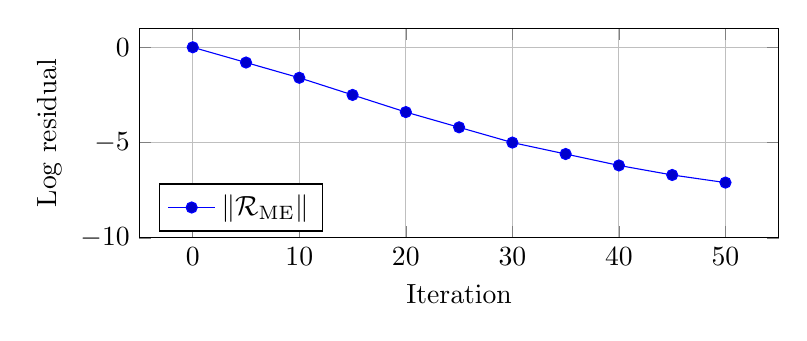
\begin{tikzpicture}
\begin{axis}[
width=0.8\textwidth,height=0.35\textwidth,
xlabel={Iteration},ylabel={Log residual},
ymin=-10,ymax=1, grid=both, legend pos=south west]
\addplot coordinates {(0,0) (5,-0.8) (10,-1.6) (15,-2.5) (20,-3.4) (25,-4.2) (30,-5.0) (35,-5.6) (40,-6.2) (45,-6.7) (50,-7.1)};
\addlegendentry{$\|\mathcal{R}_{\mathrm{ME}}\|$}
\end{axis}
\end{tikzpicture}
\caption{Placeholder: typical convergence of the master-equation residual.}
\end{figure}

\paragraph{Sanity checks.}
\begin{itemize}[leftmargin=1.25em]
\item \emph{No-price-limit case.} If $P$ is flat, the price externality vanishes. Route A and B should collapse to the same frictional-control model without cross effects.
\item \emph{Symmetric costs.} Setting $\phi_-=\phi_+$ removes the kink; $i^*$ is linear in $V_k-1$ everywhere. FP becomes smoother; residuals drop faster.
\item \emph{Elasticity sweep.} Under isoelastic demand, $\eta$ scales the externality linearly; recovered investment schedules should contract monotonically in $\eta$.
\end{itemize}

%========================
% % Economics
% %========================
\section{Economics: Aggregation, Irreversibility, Comparative Statics}

\paragraph{Aggregation.}
Aggregation enters \emph{only} via the term $e^{x+z}k^\alpha\,Y P'(Y)$ in the stationary master equation (ME). Under isoelastic demand, this is $-\eta P(Y)\,e^{x+z}k^\alpha$, which acts as a proportional reduction in marginal revenue. The mean-field externality is thus \emph{complete} and \emph{transparent}.
 

\paragraph{Comparative statics.}
\begin{itemize}[leftmargin=1.25em]
\item Larger $\eta$ (steeper demand) amplifies the negative externality, reducing investment and shifting mass in $m$ toward lower $k$.
\item Bigger $\phi_- - \phi_+$ widens irreversibility bands and slows capital reallocation, increasing dispersion in $k$ conditional on $z$.
\item Higher $\sigma_z$ spreads the cross-section in $z$, raising $Y$ volatility and, through $P'(Y)$, modulating the externality term over the business cycle.
\item Higher $\sigma_x$ (through $\Lx$) deepens precautionary effects via $r(x)$ and the HJB drift terms, with ambiguous effects on average investment depending on curvature.
\item A countercyclical $r(x)$ strengthens the value premium mechanism � la costly reversibility by raising discount rates in recessions precisely when $P'(Y)$ is most negative.
\end{itemize}

%========================
% Appendix A
%========================
\appendix
\section{Appendix A: Full Derivations and Pairings}\label{app:derivations}

\subsection{Envelope/KKT and policy recovery}
From \eqref{eq:HJB}, define $p=V_k$. The Hamiltonian
$\mathcal{H}(k,z,x,m,p)=\max_i\{\pi+p(i-\delta k)\}$
is the convex conjugate of $h$ shifted by $p-1$. The envelope condition $V_k=\partial_p \mathcal{H}$ combined with the FOC for $i$ produces the piecewise-affine policy in \Cref{prop:policy}. The kink at $p=1$ corresponds to $i=0$. KKT adds the complementary slackness $\lambda\cdot(i+\kbar(k))=0$ when a lower bound is present.

\subsection{Adjoint pairing for FP}
Let $\varphi$ be a smooth test function. Then

$$
\frac{\diff}{\diff t}\int \varphi\,\diff m_t
= \int \varphi_k (i^*-\delta k)\,\diff m_t + \int \Lz \varphi\,\diff m_t
= \int \varphi\,\diff\Big(-\partial_k[(i^*-\delta k)m_t]+\Lzadj m_t\Big).
$$

Stationarity imposes \eqref{eq:FP} with $\partial_t m=0$. Reflecting at $k=0$ eliminates the boundary integral.

\subsection{Deriving the master equation}
Consider a flow $t\mapsto (K_t,Z_t)$ for the tagged firm following control $i_t$ and a flow of measures $t\mapsto m_t$ solving \eqref{eq:FP} under the feedback $i^*(\cdot,m_t)$. By functional It�'s lemma for $U(K_t,Z_t,x,m_t)$,
\begin{align*}
\diff U &= U_k\,\diff K_t + U_z\,\diff Z_t + \tfrac12 U_{zz}\,\sigma_z^2\,\diff t \\
        &\quad + \big(\partial_t U\big|_{m}\big)\,\diff t, \\
\partial_t U\big|_{m} &= \int \Big[ (i^*(\xi,x,m)-\delta\kappa)\,\partial_{\kappa}\,\dmU
  +\mu_z(\zeta)\,\partial_{\zeta}\,\dmU
  +\tfrac12\sigma_z^2\,\partial_{\zeta\zeta}^2\,\dmU\Big] \, m(\diff \xi) \\
  &\quad + \int \delta_m \pi(\xi; k,z,x,m) \, m(\diff \xi).
\end{align*}
  where the last line uses the chain rule in \Cref{lem:chain}. Taking expectations under the pricing measure with short rate $r(x)$ and imposing stationarity produces the stationary master equation (ME).

\subsection{Externality term in detail}
Write $\pi(k,i,z,x,m)=\Psi(Y(m,x))\,\chi(k,z,x)-i-h(i,k)-f$ with $\Psi=P$ and $\chi=e^{x+z}k^\alpha$. Then

$$
\Dm\pi(m)(\xi)=\Psi'(Y)\,\chi(k,z,x)\,\chi(\kappa,\zeta,x),
$$

and integration w\.r.t.\ $m$ yields $\chi(k,z,x)\,\Psi'(Y)\,Y(m,x)$.

%========================
% Appendix B
%========================
\section{Appendix B: Residual-Loss Template (for implementation)}\label{app:loss}

For a collocation tuple $(k,z,x)$, an empirical measure $m=\tfrac1N\sum_{n=1}^N \delta_{\xi^n}$, and parameterized $U_\omega,\dmU_\psi$, define
\begin{align*}
\widehat{Y} &\equiv \frac{1}{N}\sum_{n=1}^N e^{x+\zeta^n}(\kappa^n)^\alpha,\\
\widehat{\mathcal{R}}_{\mathrm{ME}} &\equiv r(x)\,U_\omega\\
  &\quad - \max_{i}\Big\{ \pi + (U_{\omega})_k\,(i-\delta k) + \Lz U_{\omega} + \Lx U_{\omega} \Big\} \\
  &\quad - \frac{1}{N}\sum_{n=1}^N \Big[ (i^*(\xi^n,x,m)-\delta\kappa^n)\,\partial_{\kappa}\dmU_{\psi}(\xi^n)
    + \mu_z(\zeta^n)\,\partial_{\zeta}\dmU_{\psi}(\xi^n)
    + \tfrac12 \sigma_z^2\,\partial^2_{\zeta\zeta}\dmU_{\psi}(\xi^n) \Big] \\
  &\quad - e^{x+z}k^{\alpha}\,\widehat{Y}\,P'(\widehat{Y}).
  \end{align*}
  Add soft KKT penalties (one-sided around $(U_\omega)_k=1$) and boundary regularizers (reflecting $k=0$, growth at $k_{\max}$). Minimize

$$
\mathcal{L}=\E\big[\widehat{\mathcal{R}}_{\mathrm{ME}}^2\big]+\lambda_{\mathrm{KKT}}\mathcal{P}_{\mathrm{KKT}}
+\lambda_{\mathrm{bdry}}\mathcal{P}_{\mathrm{bdry}}.
$$

Anchoring $\int \dmU\,\diff m=0$ removes the gauge freedom in $\dmU$.

%========================
% Appendix C
%========================
\section{Appendix C: Common-Noise Master Equation (Reference Note)}\label{app:common-noise}

When the population law $m_t$ itself diffuses under common noise (say through an exogenous $x_t$ or an aggregate Brownian component shared by firms), the functional It� calculus on $\mathcal P_2$ introduces a second-order term in the measure variable. In a stylized form (see Carmona \& Delarue, and Cardaliaguet--Delarue--Lasry--Lions), the stationary master equation would add a term of the form

$$
\frac{1}{2}\,\Sigma_{\mathrm{com}}:\!\int\!\!\int
\partial_{\xi}\partial_{\xi'} \big(\Dm U(\xi)\big)\,\big(\Dm U(\xi')\big)
\, m(\diff \xi)\, m(\diff \xi')
$$

or, in classical PDE notation,
$\tfrac12 \mathrm{Tr}\big[\Gamma\,\partial_{\xi\xi}^2 \dmU\big]$
integrated against $m$, where $\Gamma$ is the covariance of the common noise. Because this paper conditions on $x$, these terms are absent in the stationary master equation.

%========================
% Appendix D
%========================
\section{Appendix D: Tiny Pseudocode (Plain \texorpdfstring{\texttt{listings}}{listings})}\label{app:code}

\lstset{
basicstyle=\ttfamily\small,
columns=fullflexible,
showstringspaces=false,
frame=single,
framerule=0.4pt,
breaklines=true,
tabsize=2,
captionpos=b
}

\begin{lstlisting}[language=Python,caption={Pseudo-JAX for (ME) residual with empirical measure}]

# Inputs:

# params\_omega: parameters for U(k,z,x; m)

# params\_psi:   parameters for delta\_m U(xi; k,z,x; m)

# batch:        list of tuples (k,z,x, {xi\_n=(kappa\_n,zeta\_n)}\_{n=1}^N )

# primitives:   alpha, delta, mu\_z(z), sigma\_z, mu\_x(x), sigma\_x, r(x),

# demand P(Y) and Pprime(Y), fixed cost f

# penalties:    lambdas for KKT and boundary regularizers

def policy\_from\_grad(p, k, phi\_plus, phi\_minus):
\# p = U\_k (value gradient)
if p >= 1.0:
return (k/phi\_plus)*(p - 1.0)
else:
return (k/phi\_minus)*(p - 1.0)

def reflecting\_penalty(k, i\_star):
\# discourage negative control at k=0 and large negative flux
pen0 = max(0.0, -i\_star) if k<=1e-10 else 0.0
return pen0\*\*2

def h\_cost(i, k, phi\_plus, phi\_minus):
if i >= 0.0:
return 0.5*phi\_plus*(i*i)/max(k,1e-12)
else:
return 0.5*phi\_minus\*(i\*i)/max(k,1e-12)

def HJB\_operator(k,z,x,Yhat,Uk,Uz,Uzz,Ux,Uxx,i):
q  = exp(x+z)*(k\*\*alpha)
pi = P(Yhat)*q - i - h\_cost(i,k,phi\_plus,phi\_minus) - f
return pi + Uk*(i - delta*k) + mu\_z(z)*Uz + 0.5*sigma\_z**2\*Uzz&#x20;
\+ mu\_x(x)*Ux + 0.5*sigma\_x**2\*Uxx

def ME\_residual\_for\_tuple(params\_omega, params\_psi, tup):
k,z,x,xi\_list = tup.k, tup.z, tup.x, tup.xi\_list
\# empirical measure moments
Y\_hat = mean(\[exp(x+xi.zeta)*(xi.kappa\*\*alpha) for xi in xi\_list])
\# U and its partials at (k,z,x)
U, Uk, Uz, Uzz, Ux, Uxx = U\_and\_grads(params\_omega, k,z,x, xi\_list)
\# best response i*
i\_star = policy\_from\_grad(Uk, k, phi\_plus, phi\_minus)
\# HJB maximand at i\*
H\_val  = HJB\_operator(k,z,x,Y\_hat,Uk,Uz,Uzz,Ux,Uxx,i\_star)
\# Population terms (measure derivative)
integ = 0.0
for xi in xi\_list:
dU = delta\_mU\_and\_partials(params\_psi, xi, k,z,x, xi\_list)
\# dU returns dict with fields dkappa, dzeta, dzeta2, p\_k (proxy gradient)
i\_star\_xi = policy\_from\_grad(dU\['p\_k'], xi.kappa, phi\_plus, phi\_minus)
integ += (i\_star\_xi - delta*xi.kappa)* dU\['dkappa']&#x20;
\+ mu\_z(xi.zeta)\* dU\['dzeta']&#x20;
\+ 0.5*sigma\_z\*\*2 \* dU\['dzeta2']
integ = integ / len(xi\_list)
\# direct price externality
ext  = exp(x+z)*(k\*\*alpha)\* Y\_hat \* Pprime(Y\_hat)
\# assemble residual
res  = r(x)\*U - max(H\_val, HJB\_operator(k,z,x,Y\_hat,Uk,Uz,Uzz,Ux,Uxx,0.0))&#x20;
\- integ - ext
\# penalties
pen  = reflecting\_penalty(k, i\_star)
return res, pen

def loss(params\_omega, params\_psi, batch):
sse = 0.0
pen = 0.0
for tup in batch:
res, p = ME\_residual\_for\_tuple(params\_omega, params\_psi, tup)
sse += res\*\*2
pen += p
return sse/len(batch) + lambda\_bdry\*pen
\end{lstlisting}

%========================
% Appendix E
%========================
\section{Appendix E: Symbolic Verification (PythonTeX + SymPy)}\label{app:verification}

\noindent This appendix runs minimal SymPy checks to verify key derivations used in the text. Compilation is configured (via \texttt{latexmkrc}) to execute these checks on every build; any failure triggers a build error. We assume smoothness and reflecting/no-flux boundary conditions where noted.

\begin{pyconsole}
import sympy as sp

# 1) Isoelastic simplification:  Y P'(Y) = -eta P(Y)
Y, eta = sp.symbols('Y eta', positive=True)
P = Y**(-eta)
check1 = sp.simplify(Y*sp.diff(P, Y) + eta*P)
assert check1 == 0
print("Isoelastic: Y*P'(Y) = -eta*P(Y)  [OK]")

# 2) Externality directional derivative:  d/d epsilon P(Y+epsilon*chi_eps)*chi0 |_{epsilon=0}
#     equals P'(Y) * chi0 * chi_eps
chi0, chieps, eps = sp.symbols('chi0 chieps eps', real=True)
Psi = lambda y: y**(-eta)
dpi = sp.diff(Psi(Y + eps*chieps)*chi0, eps).subs(eps, 0)
target = sp.diff(Psi(Y), Y) * chi0 * chieps
assert sp.simplify(dpi - target) == 0
print('Externality directional derivative  [OK]')

# 3) Externality, isoelastic reduction after integrating over m:  chi0 * Y * P'(Y) = -eta * P(Y) * chi0
lhs = chi0 * Y * sp.diff(Psi(Y), Y)
rhs = -eta * Psi(Y) * chi0
assert sp.simplify(lhs - rhs) == 0
print('Externality isoelastic reduction   [OK]')

# 4) KKT/FOC solution for i* with asymmetric quadratic costs
#    h = 0.5*phi_plus*i^2/k for i>=0;   0.5*phi_minus*i^2/k for i<0
i, k, p, phi_plus, phi_minus = sp.symbols('i k p phi_plus phi_minus', positive=True)
h_plus  = 0.5*phi_plus*i**2/k
FOC_plus  = sp.Eq(sp.diff(-i - h_plus + p*i, i), 0)
sol_plus  = sp.solve(FOC_plus, i)[0]
h_minus = 0.5*phi_minus*i**2/k
FOC_minus = sp.Eq(sp.diff(-i - h_minus + p*i, i), 0)
sol_minus = sp.solve(FOC_minus, i)[0]
assert sp.simplify(sol_plus  - k*(p-1)/phi_plus)  == 0
assert sp.simplify(sol_minus - k*(p-1)/phi_minus) == 0
print('KKT/FOC piecewise i* formulas     [OK]')

# 5) FP adjoint pairing identity (algebraic, boundary terms omitted):
#    phi_k * (a*m) = d_k(phi*a*m) - phi * d_k(a*m)
kk = sp.symbols('kk', real=True)
phi = sp.Function('phi')(kk)
a   = sp.Function('a')(kk)
mm  = sp.Function('m')(kk)
expr = sp.diff(phi, kk)*(a*mm) - (sp.diff(phi*(a*mm), kk) - phi*sp.diff(a*mm, kk))
assert sp.simplify(expr) == 0
print('Adjoint pairing identity (no-flux) [OK]')

# 6) Envelope property for Hamiltonian in p: d/dp max_i { -i - h(i,k) + p i } = i*(p)
#    Check separately on each branch (ignoring terms not depending on i, e.g., -delta*k*p)
H_plus  = (-i - h_plus + p*i).subs(i, sol_plus)
H_minus = (-i - h_minus + p*i).subs(i, sol_minus)
dHp_dp  = sp.simplify(sp.diff(H_plus, p))
dHm_dp  = sp.simplify(sp.diff(H_minus, p))
assert sp.simplify(dHp_dp - sol_plus) == 0
assert sp.simplify(dHm_dp - sol_minus) == 0
print('Envelope: dH/dp equals i*(p)       [OK]')

print('\nAll SymPy verification checks passed.')
\end{pyconsole}

%========================
% Bibliography (manual)
%========================
\begin{thebibliography}{99}\small

\bibitem{carmona_delarue_2018_mfg} Carmona, R. and F. Delarue (2018).
\emph{Probabilistic Theory of Mean Field Games with Applications.}
Springer.

\bibitem{cardaliaguet_delarue_lasry_lions_2019} Cardaliaguet, P., F. Delarue, J.-M. Lasry, and P.-L. Lions (2019).
\emph{The Master Equation and the Convergence Problem in Mean Field Games.}
Princeton University Press.

\bibitem{lasry_lions_2007} Lasry, J.-M. and P.-L. Lions (2007).
Mean field games.
\emph{Japanese Journal of Mathematics} 2(1): 229--260.

\bibitem{mou_zhang_cn_master} Mou, C.-H. and J. Zhang (various years).
Second-order master equations with common noise and displacement monotonicity.
(Working papers / journal articles; see also related notes by Gangbo--M�sz�ros--Mou--Zhang.)

\bibitem{zhang_2005_value_premium} Zhang, L. (2005).
The value premium.
\emph{Journal of Finance} 60(1): 67--103.

\end{thebibliography}

\end{document}

